\documentclass[]{book}
\usepackage[english]{babel}
\usepackage[utf8]{inputenc}
\usepackage{fancyhdr}
\usepackage{graphicx}
\pagestyle{fancy}
\fancyhf{}
\rhead{
\includegraphics[width=2cm, height=1cm]{logo}}
\lhead{Python Programming :: Unit 1}
\lfoot{COPYRIGHT ©TALENTSPRINT, 2020. ALL RIGHTS RESERVED.}
\rfoot{\thepage}
\begin{document}
    \Section*{Tool Chain}
    There are many ways to create Python programs:
    \paragraph {1. Interactive Interpreter} ~
    \begin{itemize}
        \item You can start the interpreter just by giving the name python3 or python
        \item Once Python has started, you will see the interpreter startup message indicating version and platform and be given the interpreter prompt \emph{$>>>$} to enter commands.
    \end{itemize}
    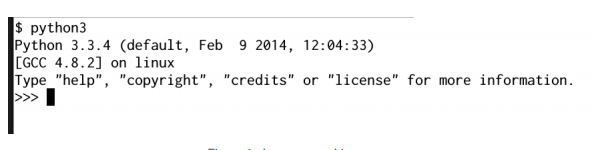
\includegraphics{interpreter}
    \paragraph {2. Writing Script on file} Follow these steps to write and execute a script
    \begin{itemize}
        \item At the (\$) prompt create a file using vim (or any text editor), \\
            vim filename.py

        \item Write code in the file save it
        \item Execute - come back to terminal and type $ python filename.py it generates the output in the console
    \end{itemize}
    As you can gather python programs have the extension .py
    \paragraph {3.Integrated Development Environment} We can also use graphical Interactive Development Environment - IDE to enter, and run python programs. The default ide in Linux is called IDLE. 
    
    IDLE is the basic editor and interpreter environment with standard distribution of python. It looks like,
    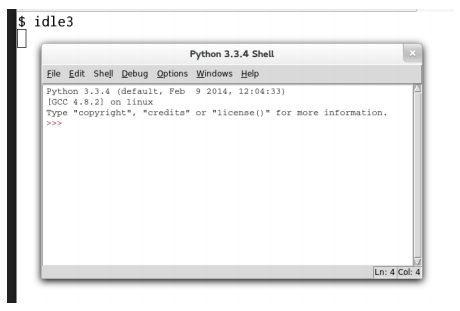
\includegraphics{idle}
    \paragraph {4. Using iPython} Our preferrred interactive environment is called iPython. It is invoked by typing ipython3 at the \$ prompt.
    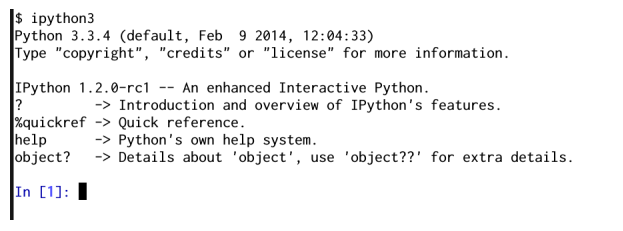
\includegraphics{ipython}
    \section*{HelloWorld Program}
    Now let us write our first Python program. The program will display a message: HelloWorld
    
    Let us open the terminal and run the python interpreter: that is type python3 at the \$prompt.
    
    At the \emph{$>>>$} prompt type the line (and hit ENTER).

    \emph{$>>>$ print("HelloWorld!!")}
    
    It produces the following result:
    
    HelloWorld!!

    Now let us write the same program in a script

    \begin{itemize}
        \item Open the file using $ vim Program-01-1.py and type the following line and save the file. \\
                print("HelloWorld!!")
        \item Now type the below command in terminal and press Enter Key to Execute.
                \emph{\$ python Program-01-1.py}
    \end{itemize}
    \paragraph{Note:} Recall that python is an interpreted language. So the execution takes place without any compiling, linking or producing an executable.
\end{document}
